% !TEX root = collection.tex

\chapter{Zero-Knowledge Proofs}
Traditional Euclidean style proofs allow us to prove veracity of statements to others. However, such proof systems have two shortcomings: (1) the running time of the verifier needs to grow with the length of the proof, and (2) the proof itself needs to be disclosed to the verifier. In this chapter, we will provide methods enabling provers to prove veracity of statements of their choice to verifiers while avoiding the aforementioned limitations. In realizing such methods we will allow the prover and verifier to be probabilistic and also allow them to interact with each other.\footnote{Formally, they can be modeled as interactive PPT Turing Machines.}

\section{Interactive Proofs}
		{\definition {\normalfont\textbf{(Interactive Proof System)}} For a language L we have an \textit{interactive proof system} if $\exists$ a pair of algorithms (or better, interacting machines) $(\mathcal{P},\mathcal{V})$, where $\mathcal{V}$ is polynomial in $|x|$, and both can flip coins, such that:
		\begin{itemize}
			\item Completeness: $\forall x\in L$
		$$\Pr_{\mathcal{P},\mathcal{V}} \left[Output_{\mathcal{V}}(\mathcal{P}(x) \leftrightarrow \mathcal{V}(x))=1\right]=1,$$
			\item Soundness: $\forall x\notin L$, $\forall \mathcal{P}^*$
		$$\Pr_{\mathcal{V}} \left[Output_{\mathcal{V}}(\mathcal{P}^*(x) \leftrightarrow \mathcal{V}(x))=1\right]<neg(|x|),$$
		\end{itemize} where $Output_{\mathcal{V}}(\mathcal{P}(x) \leftrightarrow \mathcal{V}(x))$ denotes the output of $\mathcal{V}$ in the interaction between $\mathcal{P}$ and $\mathcal{V}$ where both parties get $x$ as input.
		We stress that $\mathcal{P}$ and $\mathcal{P}^*$ can be computationally unbounded. }



\paragraph{Interactive Proof for Graph Non-Isomorphism (GNI).} We say that two graphs $G_0$ and $G_1$ are isomorphic, denoted $G_0 \cong G_1$, if $\exists$ an isomorphism $f: V(G_0) \rightarrow V(G_1)$ s.t. $(u,v)\in E(G_0)$ iff $(f(u),f(v))\in E(G_1)$, where $V(G)$ and $E(G)$ are the vertex and edge sets of some graph $G$. On the other hand, $G_0$ and $G_1$ are said to be non-isomorphic, $G_0 \ncong G_1$, if $\nexists$ any such $f$, and $GNI=\lbrace(G_0,G_1)|\  G_0\ncong G_1\rbrace$ be the language that consists of pairs of graphs that are not isomorphic. 

GNI is not believed to have short proofs so an interactive proof could offer a prover a mechanism to prove to a polynomially bounded verifier that two graphs are non-isomorphic. 


The intuition behind a protocol to accomplish the above task is simple. Consider a verifier that randomly rename the vertices of one of the graphs and give it to the prover. Can the prover given the relabeled graph figure out which graph did the verifier start with?  If $G_0$ and $G_1$ were not isomorphic  then an unbounded prover can figure this out. However, in case $G_0$ and $G_1$ {are} isomorphic then the distribution resulting form random relabelings of $G_0$ and $G_1$ are actually identical. Therefore, even an unbounded prover has no way of distinguishing which graph the verifier started with. So the prover has only a $\frac12$ probability of guessing which graph the verifier started with. Note that by repeating this process we can reduce the success probability of a cheating prover to negligible. More formally:

%		If they consistently answer correctly, however, it would be hard to remain skeptical against $G_0 \ncong G_1$ as they beat the odds to almost impossible limits.  And so this interaction can ``prove" very strongly to the verifier that $(G_0,G_1)\in$ GNI.  Consider the protocol we can define from this:

		\begin{center}
			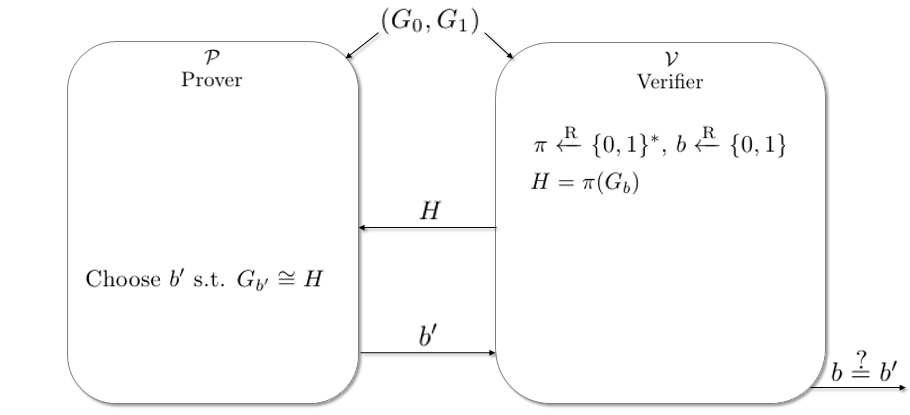
\includegraphics[scale=.51094]{GNI_IP_Protocol.png}
		\end{center}

		\begin{itemize}
			\item Completeness: If $(G_0,G_1)\in$ GNI, then the unbounded $\mathcal{P}$ can distinguish isomorphism of $G_0$ against those of $G_1$ and can always return the correct $b'$.  Thus, $\mathcal{V}$ will always output 1 for this case.
			\item Soundness: If $(G_0,G_1)\notin$ GNI, then it is equiprobable that $H$ is a random isomorphism of $G_0$ as it is $G_1$ and so $\mathcal{P}$'s guess for $b'$ can be correct only with a probability $\frac{1}{2}$.  Repeating this protocol $k$ times means the probability of guessing the correct $b'$ for all $k$ interactions is $\frac{1}{2^k}$.  And so the probability of $\mathcal{V}$ outputting 0 (e.g. rejecting $\mathcal{P}$'s proof at the first sign of falter) is $1-\frac{1}{2^k}$. 
		\end{itemize}

		%The interaction between prover and verifier captures the notion of a proof system for GNI, a problem previously not known to have an efficient method of proof.  By interacting, we can prove what seemed impossible to efficiently prove before!


\section{Zero Knowledge Proofs}


{\definition {\normalfont\textbf{(NP-Verifier)}} A language L has an NP-verifier if $\exists$ a verifier $\mathcal{V}$ that is polynomial time in $|x|$ such that:
		\begin{itemize}
			\item Completeness: $\forall x\in L,\ \exists\ a\ proof\ \pi\ s.t.\ \mathcal{V}(x,\pi)=1$
			\item Soundness: $\forall x \notin L$ $\forall$ purported proof $\pi$ we have $\mathcal{V}(x,\pi)=0$
		\end{itemize}}

		That is, the conventional idea of a proof is formalized in terms of what a computer can efficiently verify.  So a set of statements considered true (e.g. in a language $L$) is complete and sound if a proof can be written down that can be ``easily" and rigorously verified if and only if a statement is in the language.


\bigskip
\noindent\textbf{Efficient Provers.}
		Unfortunately (fortunately?), there aren't real-life instances of all-powerful provers that we know of.  And for cryptography we must make more reasonable assumptions about the provers.  In this case we will assume provers are also bounded to be \emph{efficient}.
		
		Previously, if a prover wanted to prove that two graphs, $G_0$ and $G_1$ were isomorphic, it would use its all-powerfulness to find the isomorphic mapping between the two graphs and give it to the verifier to complete the proof.  But now, being computationally bounded, the prover is in the same boat as the verifier and can find a proof no better than the verifier can.  In order for the prover to be able to prove something that the verifier cannot find out on their own, the prover must have some extra information.  If, for example, the prover simply knew the isomorphism between the graphs, this would be the sufficient extra information it needs to enact the proof.  That's a rather boring proof though.  We have interaction now!  Can't we do something fancier?
		
		What if the prover wanted to prove that two graphs were isomorphic but didn't want to fully reveal the isomorphism that they know.  If they're lying and don't know an isomorphism is their a way we can exploit them again?
		
		When $G_0$ and $G_1$ are isomorphic, the isomorphism between them would be a \textit{witness}, $w$, to that fact, that can be used in the proof.  Unfortunately, the prover is being stubborn and won't just tell us that isomorphism, $w:V(G_0)\rightarrow V(G_1)$, that they claim to have.  The prover is comfortable however giving us a ``scrambled" version, $\phi$, of $w$ as long as it doesn't leak any information about their precious $w$.  For example, the prover is willing to divulge $\phi = \pi \circ w$ where $\pi$ is a privately chosen random permutation of $|V|=|V(G_0)|=|V(G_1)|$ vertices.  Since $\pi$ renames vertices completely randomly, it scrambles what $w$ is doing entirely and $\phi$ is just a random permutation of $|V|$ elements.  At this point, we might be a little annoyed at the prover since we could have just created a random permutation on our own.  This might give us an idea on how to gain a little more information however, even though we gained none here:
		
		If we want to be convinced that $\phi$ really is of the form $\pi \circ w$, thus containing $w$ in its definition, and isn't just a completely random permuation, we can note that if it is of that form then $\phi(G_0)=\pi(w(G_0))=\pi(G_1)$ (since $w$ being an isomorphism implies that $w(G_0)=G_1$).  Note that we started with a mapping on input $G_0$ and ended with a mapping on input $G_1$.  With an isormphism, one could get from one graph to the other seamlessly; if the prover \textit{really} has the isomorphism it claims to have, then it should have no problem displaying this ability.  So, what if we force the prover to give us $H=\pi (G_1)$ just after randomly choosing its $\pi$ and then let it show us its ability to go from $G_1$ to $G_0$ with ease: give us a $\phi$ so that $\phi(G_0)=\pi(G_1)=H$.  The only way the prover can give a mapping that jumps from $G_0$ to $G_1$ in such a way is if they know an isomorphism; if the prover could find a $\phi$ efficiently but did \textit{not} know an isomorphism then they would have been able to see that $\pi^{-1}(\phi(G_0))=G_1$ and thus have $\pi^{-1}\circ\phi$ as an isomorphism from $G_0$ to $G_1$, which would contradict the assumed hardness of finding isomorphisms in the GI problem.  So by forcing the prover to give us $H$ as we've defined and to produce a $\phi$ so that $\phi(G_0)=H$, we've found a way to expose provers that don't really have an isomorphism and we can then be convinced that they really do know $w$ when they pass our test.  And the prover didn't directly tell us $w$, so they may be able to salvage some secrecy!
		
		But not everything is airtight about this interaction.  Why, for instance, would the prover be willing to provide $H=\pi(G_1)$ when they're trying to divulge as little information as possible?  The prover was comfortable giving us $\phi$ since we could have just simulated the process of getting a completely random permutation of vertices ourselves, but couldn't the additional information of $H$ reveal information about $w$?  At this point, the annoyed feeling may return as we realize that, $H=\pi(G_1)=\pi'(G_0)$, for some $\pi'$, is just a random isomorphic copy of $G_0$ \textit{and} $G_1$ as long as $G_0 \cong G_1$; we could have just chosen a random $\pi'$, set $H=\pi'(G_0)$, and let $\phi=\pi'$ and would have created our very own random isomorphic copy, $H$, of $G_1$ that satisfies our test condition $H=\phi(G_0)$ just like what we got from our interaction with the prover.  We couldn't have gained any new information from the prover because we could have run the whole test on our own!
		
		Well, something must be wrong; we couldn't have been convinced of something without gaining \textit{any} new information.  Indeed, the test has a hole in it: how can we force the prover to give us $H=\pi(G_1)$ like we asked?  If the prover is lying and it knows our test condition is to verify that $H=\phi(G_0)$, the prover might just cheat and give us $H=\pi(G_0)$ so it doesn't have to use knowledge of $w$ to switch from $G_1$ to $G_0$.  And, in fact, by doing this and sending $\phi=\pi$, the prover would fool us!
		
		To keep the prover on their toes, though, we can randomly switch whether or not we want $H$ to equal $\phi(G_0)$ or $\phi(G_1)$.  If, in our interaction, the prover must first provide their $H=\pi(G_1)$ before we let them know which we want, they then lock themselves into a commitment to either $G_0$ or $G_1$ depending on whether they're trying to cheat or not, respectively.  They only have a $50\%$ chance of committing to the same case we want on a given round and so, if they don't have $w$ to deftly switch between $G_0$ and $G_1$ to always answer correctly, they again have to be an extremely lucky guesser if they're trying to lie.
		
		Again, we've created an interactive scheme that can catch dishonest provers with probability 1-$\frac{1}{2^k}$ and where we always believe honest provers!
		
		\begin{center}
			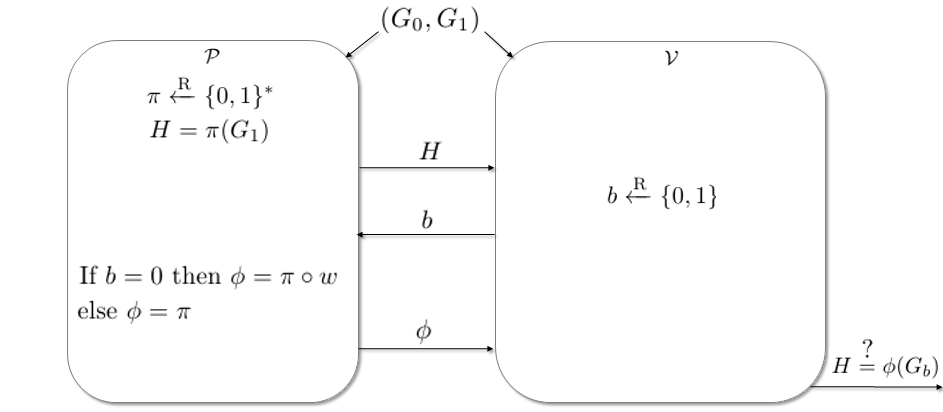
\includegraphics[scale=.51094]{GI_ZK_Protocol.png}
		\end{center}
		
		\begin{itemize}
			\item Completeness: If $(G_0,G_1)\in$ GI and $\mathcal{P}$ knows $w$, then whether $\mathcal{V}$ chooses $b=0$ or 1, $\mathcal{P}$ can always give the correct $\phi$ which, by definition, will always result in $H=\phi(G_b)$ and so $\mathcal{V}$ will always output 1.
			\item Soundness: If $(G_0,G_1)\notin$ GI, then $\mathcal{P}$ can only cheat, as discussed earlier, if the original $H$ it commits to ends up being $\pi(G_b)$ for the $b$ that is randomly chosen at the next step.  Since $b$ isn't even chosen yet, this can only happen by chance with probability $\frac{1}{2}$.  And so the probability $\mathcal{V}$ outputs 0 is $1-\frac{1}{2^k}$ for $k$ rounds.
		\end{itemize}
		
		And so, again, we've correctly captured the idea of a proof by having this interaction.  But there's a strange feeling that may be lingering around us...
		
		As a verifier, we've seen some things in interacting with the prover.  Surely, clever folks like ourselves must be able to glean \textit{some} information about $w$ after seeing enough to thoroughly convince us that the prover knows $w$.  We've first seen $H$, and we've also seen the random $b$ that we chose, along with $\phi$ at the end;  this is our whole view of information during the interaction.  But we're more bewildered than annoyed this time when we realize we could have always just chosen $b$ and $\phi$ randomly and set $H=\phi(G_b)$ on our own.  Again, everything checks out when $G_0 \cong G_1$ and we could have produced everything that we saw during the interaction before it even began.  That is, the distribution of the random variable triple ($H$, $b$, $\phi$) is identical whether it is what we saw from the prover during the interaction or it is yielded from the solitary process we just described.  We've just constructed a complete interactive proof system that entirely convinces us of the prover's knowledge of $w$, yet we could have simulated the whole experience on our own!  We couldn't have gain any knowledge about $w$ since we didn't see anything we couldn't have manufactured on own, yet we are entirely convinced that $(G_0,G_1)\in$ GI and that $\mathcal{P}$ knows $w$!  And so the prover has proven something to us yet has given us absolutely zero additional knowledge!
		
		This may feel very surprising or as if you've been swindled by a fast talker, and it very much should feel this way; it was certainly an amazing research discovery!  But this is true, and it can be made rigorous:
		
		We should first be sure what we want out of this new proof system.  We of course want it to be complete and sound so that we accept proofs iff they're true.  But we also want the verifier to gain zero knowledge from the interaction; that is, the verifier should have been able to simulate the whole experience on its own without the verifier.
		Finally, we would also like all witnesses to a true statement to each be sufficient to prove the veracity of that statement and so we let $R$ be the relation s.t. $x \in L$ iff $\exists$ a witness $w$ s.t. $(x,w)\in R$.  We can then gather all witness by defining $R(x)$ to be the set of all such witnesses.
		
		{\definition {\normalfont\textbf{(Honest Verifier Zero Knowledge Proof [HVZK])}} For a language L we have a (perfect) \textit{HVZK proof system} w.r.t. witness relation $R$ if $\exists$ an interactive proof system, $(\mathcal{P},\mathcal{V})$ s.t. $\exists$ a PPT machine $\mathcal{S}$ (called the simulator) s.t. $\forall x \in L$, $\forall w\in R(x)$ the following distributions are identical:
		$$View_{\mathcal{V}}(\mathcal{P}(x,w) \leftrightarrow \mathcal{V}(x))$$
		$$\mathcal{S}(x)$$
		where $View_{\mathcal{V}}(\mathcal{P}(x,w) \leftrightarrow \mathcal{V}(x))$ is the random coins of $\mathcal{V}$ and all the messages $\mathcal{V}$ saw.}

\begin{remark}
In the above definition, $View_{\mathcal{V}}(\mathcal{P}(x,w) \leftrightarrow \mathcal{V}(x))$ contains both the random coins of $\mathcal{V}$ and all the messages that $\mathcal{V}$ saw, because they together constitute the view of $\mathcal{V}$, and they are correlated. If the random coins of $\mathcal{V}$ are not included in the definition of $View_{\mathcal{V}}(\mathcal{P}(x,w) \leftrightarrow \mathcal{V}(x))$, then even if $\mathcal{S}$ can generate all messages that $\mathcal{V}$ saw with the same distribution as in the real execution, the verifier may still be able to distinguish the two views using its random coins.
\end{remark}
		
		There is an interesting progression of the requirements of a proof system: Completeness, Soundness, and the Zero Knowledge property.  Completeness first cares that a prover-verifier pair exist and can capture all true things as a team that works together; they both honestly obey the protocol trying prove true statements.  Soundness, however, assumes that the prover is a liar and cares about having a strong enough verifier that can stand up to any type of prover and not be misled.  Finally, Zero Knowledge assumes that the verifier is hoping to glean information from the proof to learn the prover's secrets and this requirement makes sure the prover is clever enough that it gives no information away in its proof.
		
		Unlike the soundness' requirment for a verifier to combat \textit{all} malicious provers, HVZK is only concerned with the verifier in the original prover-verifier pair that follows the set protocol.  Verifiers that stray from the protocol or cheat, however, are captured in the natural generalization to Zero Knowledge proofs.  
%		These are mostly discussed (including auxiliary inputs) in the next class, although the first definition is given below:
%		
%		{\definition {\normalfont\textbf{(Zero Knowledge Proof [ZK])}} For a language L we have a (perfect) \textit{ZK proof system} w.r.t. witness relation $R$ if $\exists$ an interactive proof system, $(\mathcal{P},\mathcal{V})$ s.t. $\exists$ a PPT machine $\mathcal{S}$ (called the simulator) s.t. $\forall x \in L$, $\forall w\in R(x)$, $\forall \mathcal{V}^*$, the following distributions are identical:
%		$$View_{\mathcal{V}^*}(\mathcal{P}(x,w) \leftarrow \mathcal{V}^*(x))$$
%		$$\mathcal{S}^{\mathcal{V}^*}(x)$$
%		where $\mathcal{S}^{\mathcal{V}^*}(x)$ is the simulator with oracle access to $\mathcal{V}^*$.}

